%%%%%%%%%%%%%%%%%%%%%%%%%%%%%%%%%%%%%%%%%%%%%%%%%%%%%%%%%%%%%%%%%%%%%%%%%%%%%%%%%%%%%%%%%%%%%%%%%%%%%%%%%%%%%%%%%%%%%%%%%%%%%%%%%%%%%%%%%%%%%%%%%%%%%%%%%%%
% This is just an example/guide for you to refer to when producing your supplementary material for your Frontiers article.                                 %
%%%%%%%%%%%%%%%%%%%%%%%%%%%%%%%%%%%%%%%%%%%%%%%%%%%%%%%%%%%%%%%%%%%%%%%%%%%%%%%%%%%%%%%%%%%%%%%%%%%%%%%%%%%%%%%%%%%%%%%%%%%%%%%%%%%%%%%%%%%%%%%%%%%%%%%%%%%

%%% Version 2.5 Generated 2018/06/15 %%%
%%% You will need to have the following packages installed: datetime, fmtcount, etoolbox, fcprefix, which are normally inlcuded in WinEdt. %%%
%%% In http://www.ctan.org/ you can find the packages and how to install them, if necessary. %%%
%%%  NB logo1.jpg is required in the path in order to correctly compile front page header %%%

\documentclass[utf8]{frontiers_suppmat} % for all articles
\usepackage{url,hyperref,lineno,microtype}
\usepackage[onehalfspacing]{setspace}



% Leave a blank line between paragraphs instead of using \\

\begin{document}
\onecolumn
\firstpage{1}

\title {{\helveticaitalic{Supplementary Material}}}


\maketitle


\section{Supplementary Data}



\subsection{Figures}

%%% There is no need for adding the file termination, as long as you indicate where the file is saved. In the examples below the files (logo1.eps and logos.eps) are in the Frontiers LaTeX folder
%%% If using *.tif files convert them to .jpg or .png
%%%  NB logo1.eps is required in the path in order to correctly compile front page header %%%

\begin{figure}[h]
	\begin{center}
		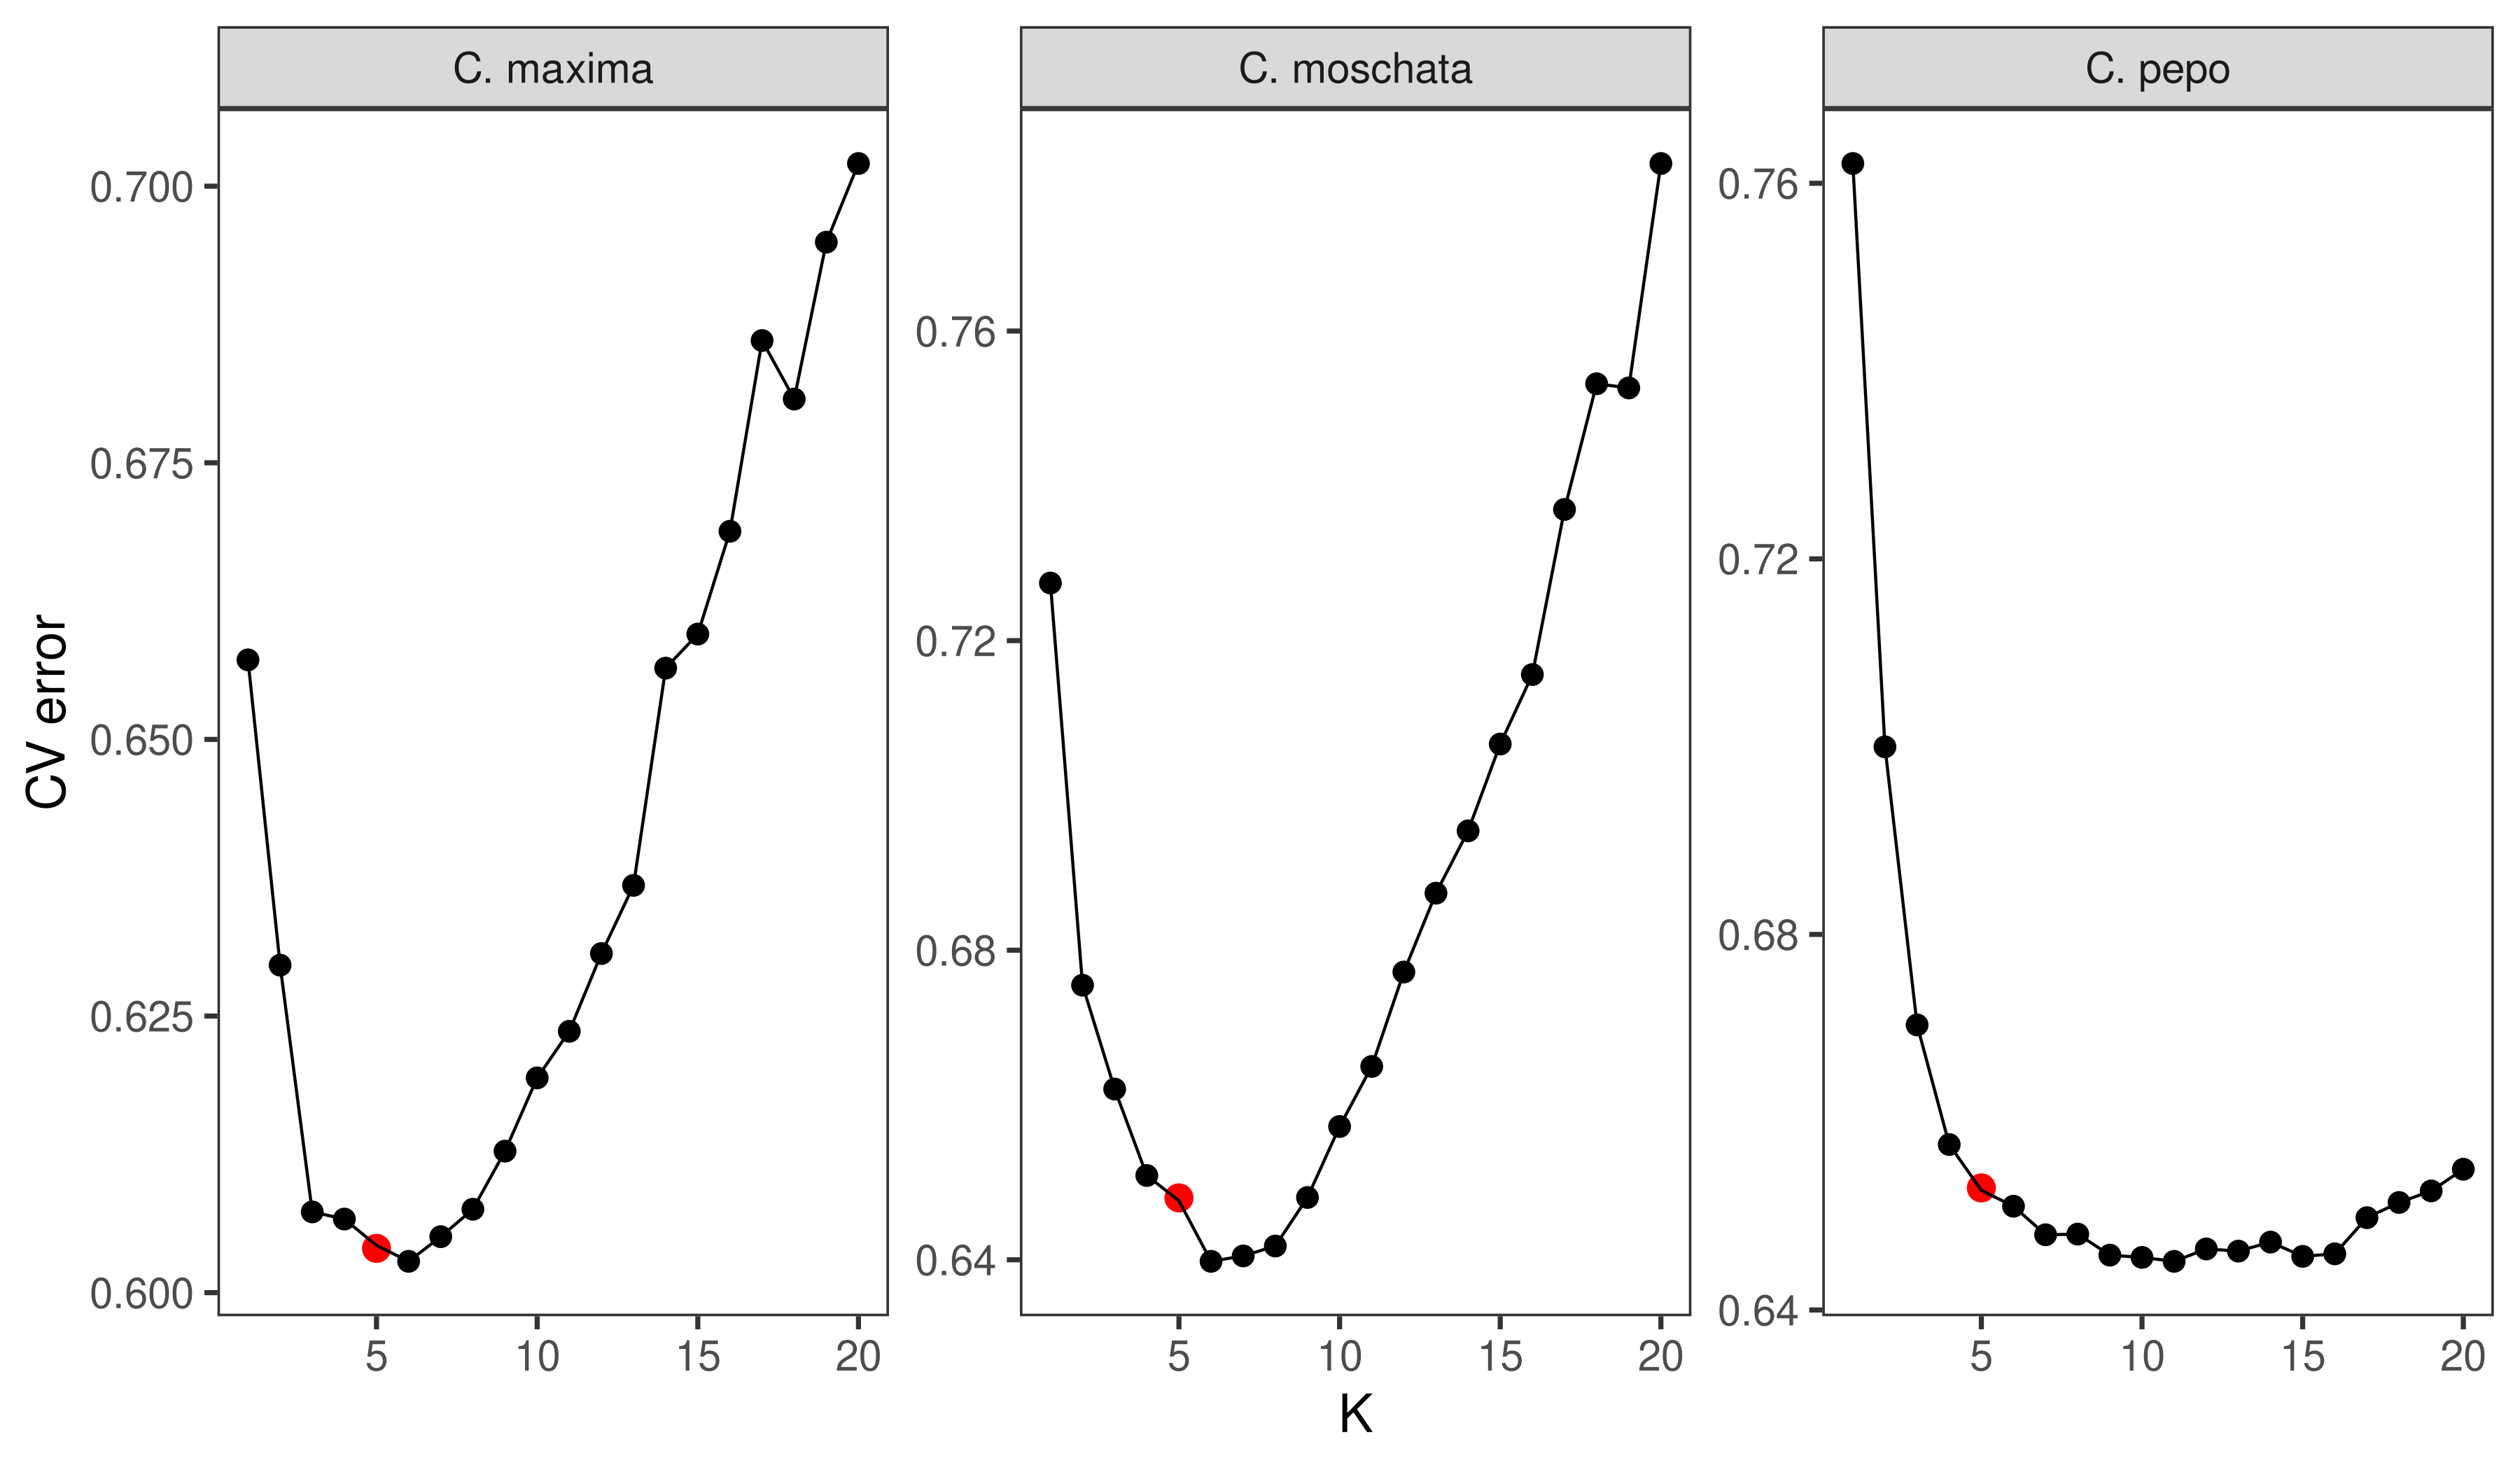
\includegraphics[width=\textwidth]{../supplemental/02_fig.png}
	\end{center}
	\caption{Geographical distribution of the USDA \textit{Cucurbita} ssp. collection. The size of the pie chart is scaled according to the number of accessions. Sector areas correspond to the proportion of the three species. \label{fig:1}}
\end{figure}


\begin{figure}[h]
\begin{center}
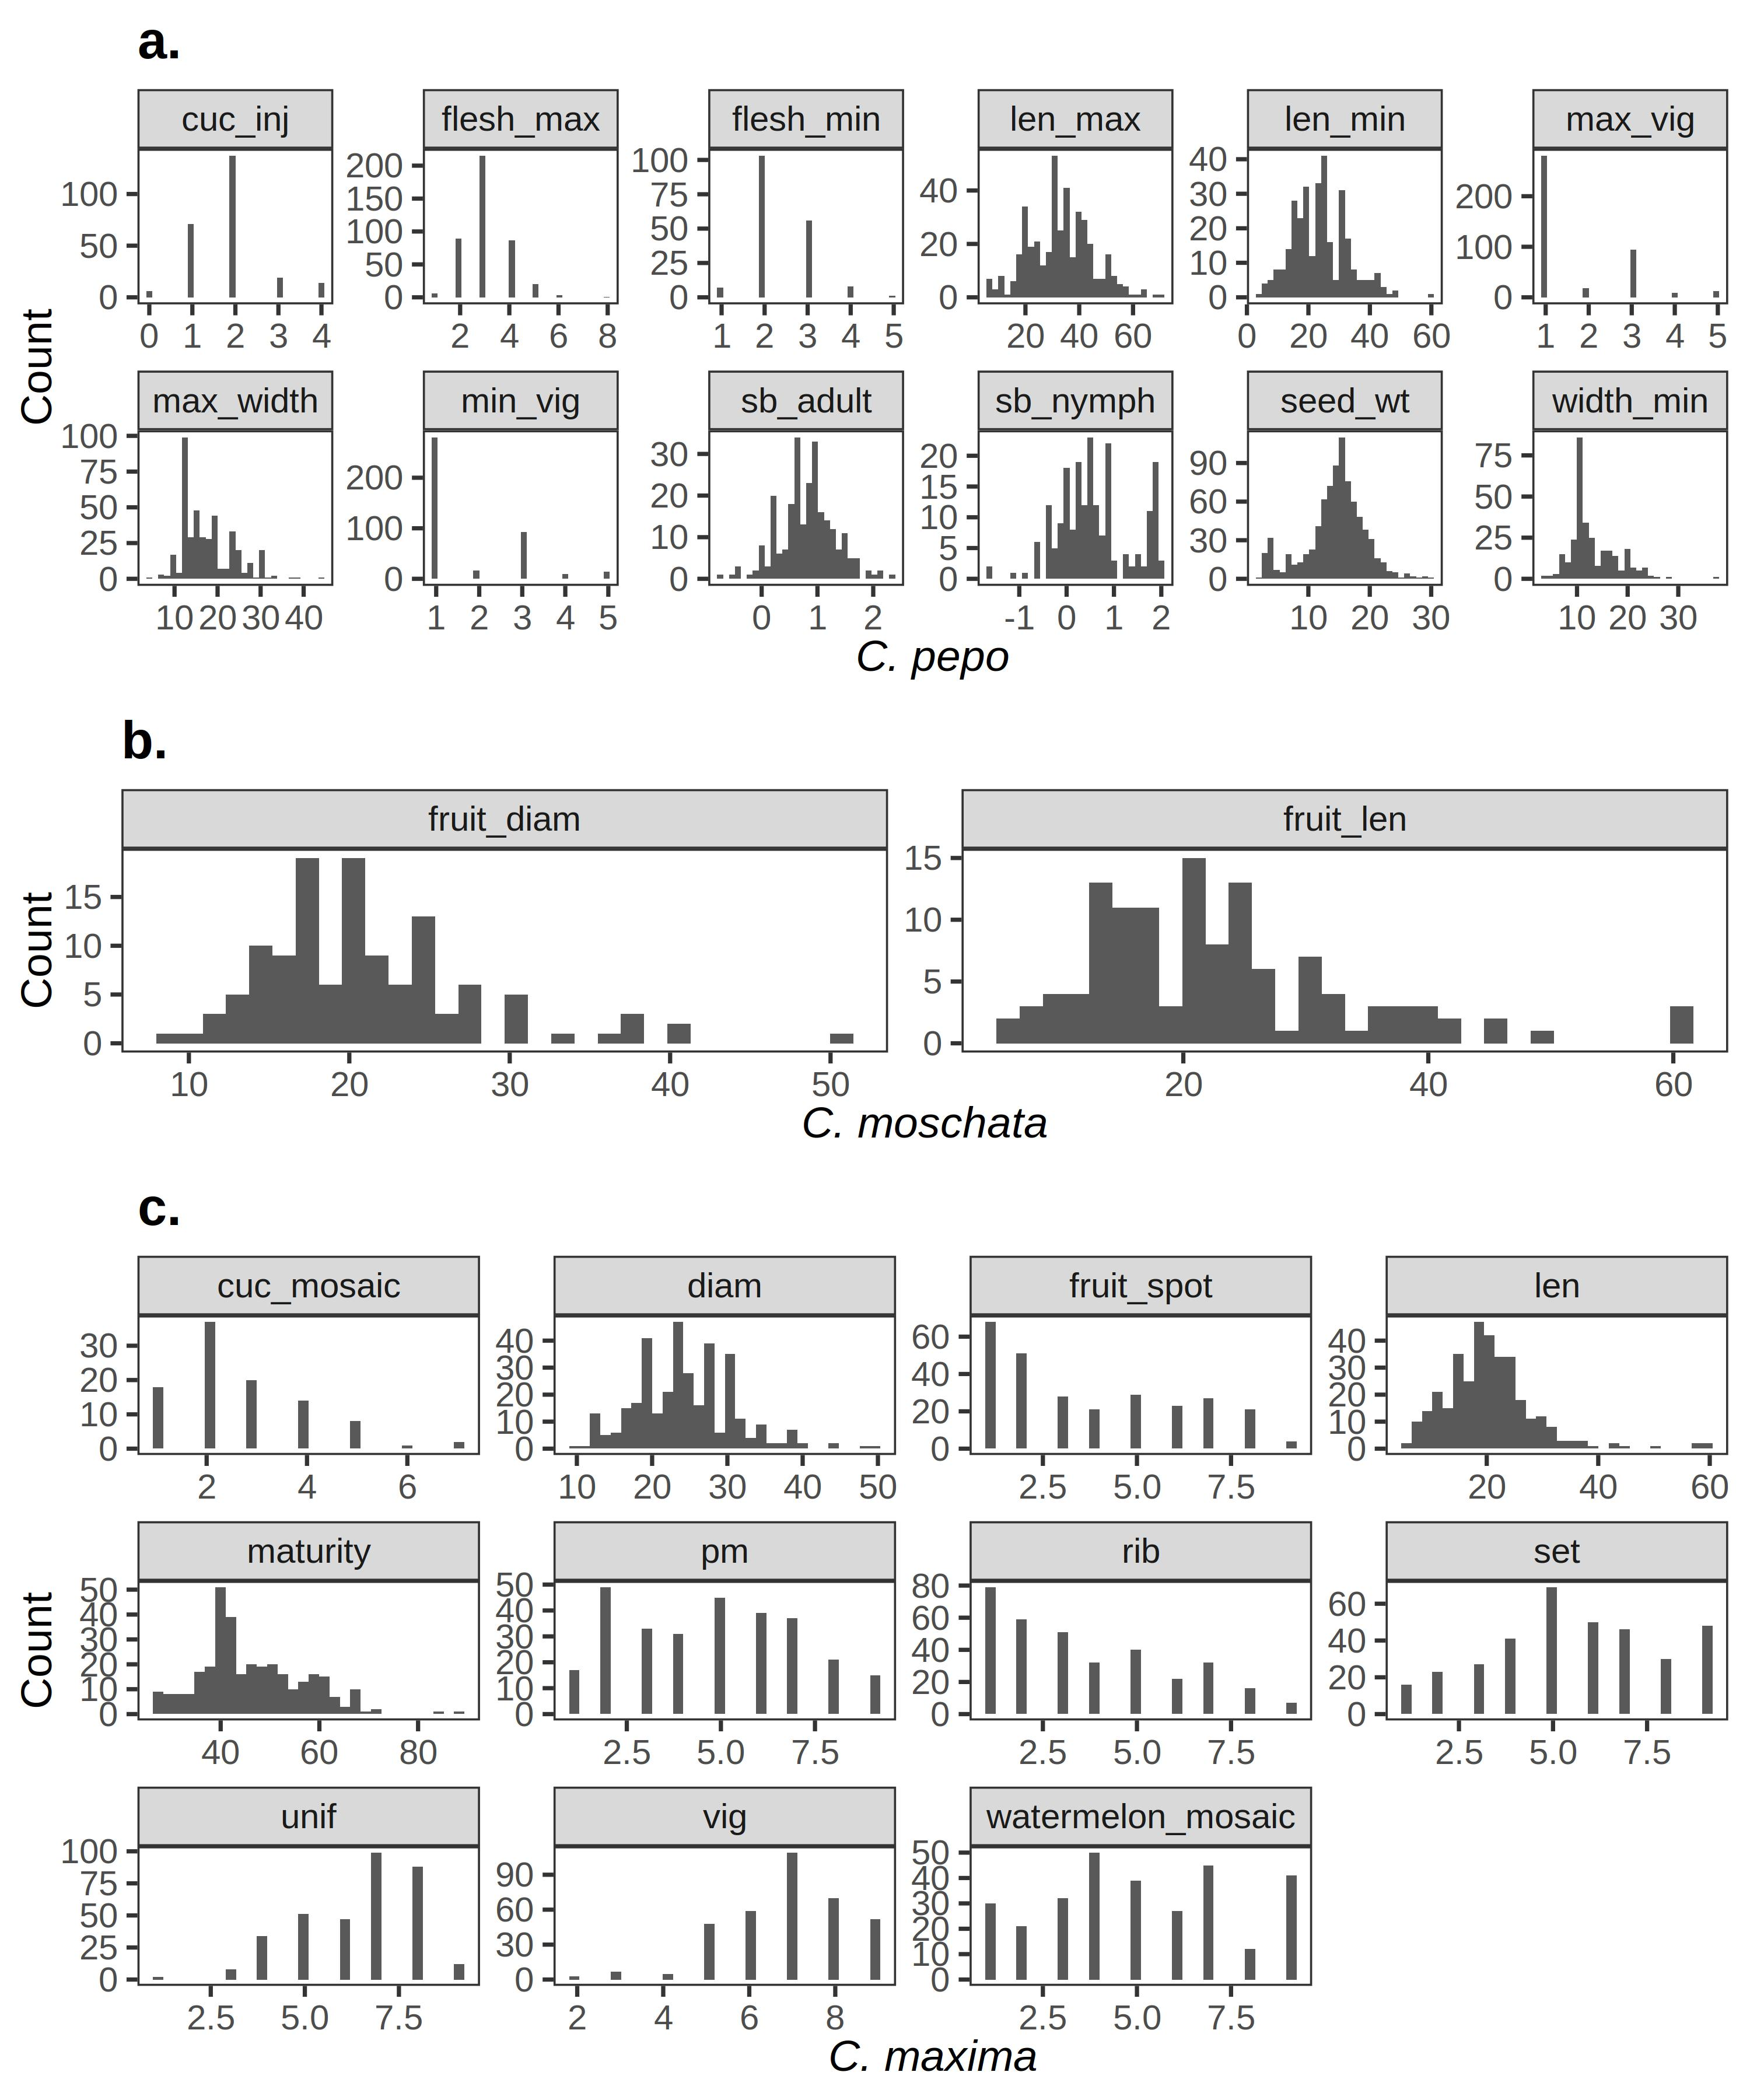
\includegraphics[width=0.8\textwidth]{../supplemental/01_supfig}% This is a *.eps file
\end{center}
\caption{Histograms of continuous and ordinal traits for \textbf{Panel a.} \textit{C. pepo}, \textbf{Panel b.} \textit{C. moschata}, and \textbf{Panel c.} \textit{C. maxima.}\label{fig:1}}
\end{figure}

\clearpage

\begin{figure}[h]
	\begin{center}
		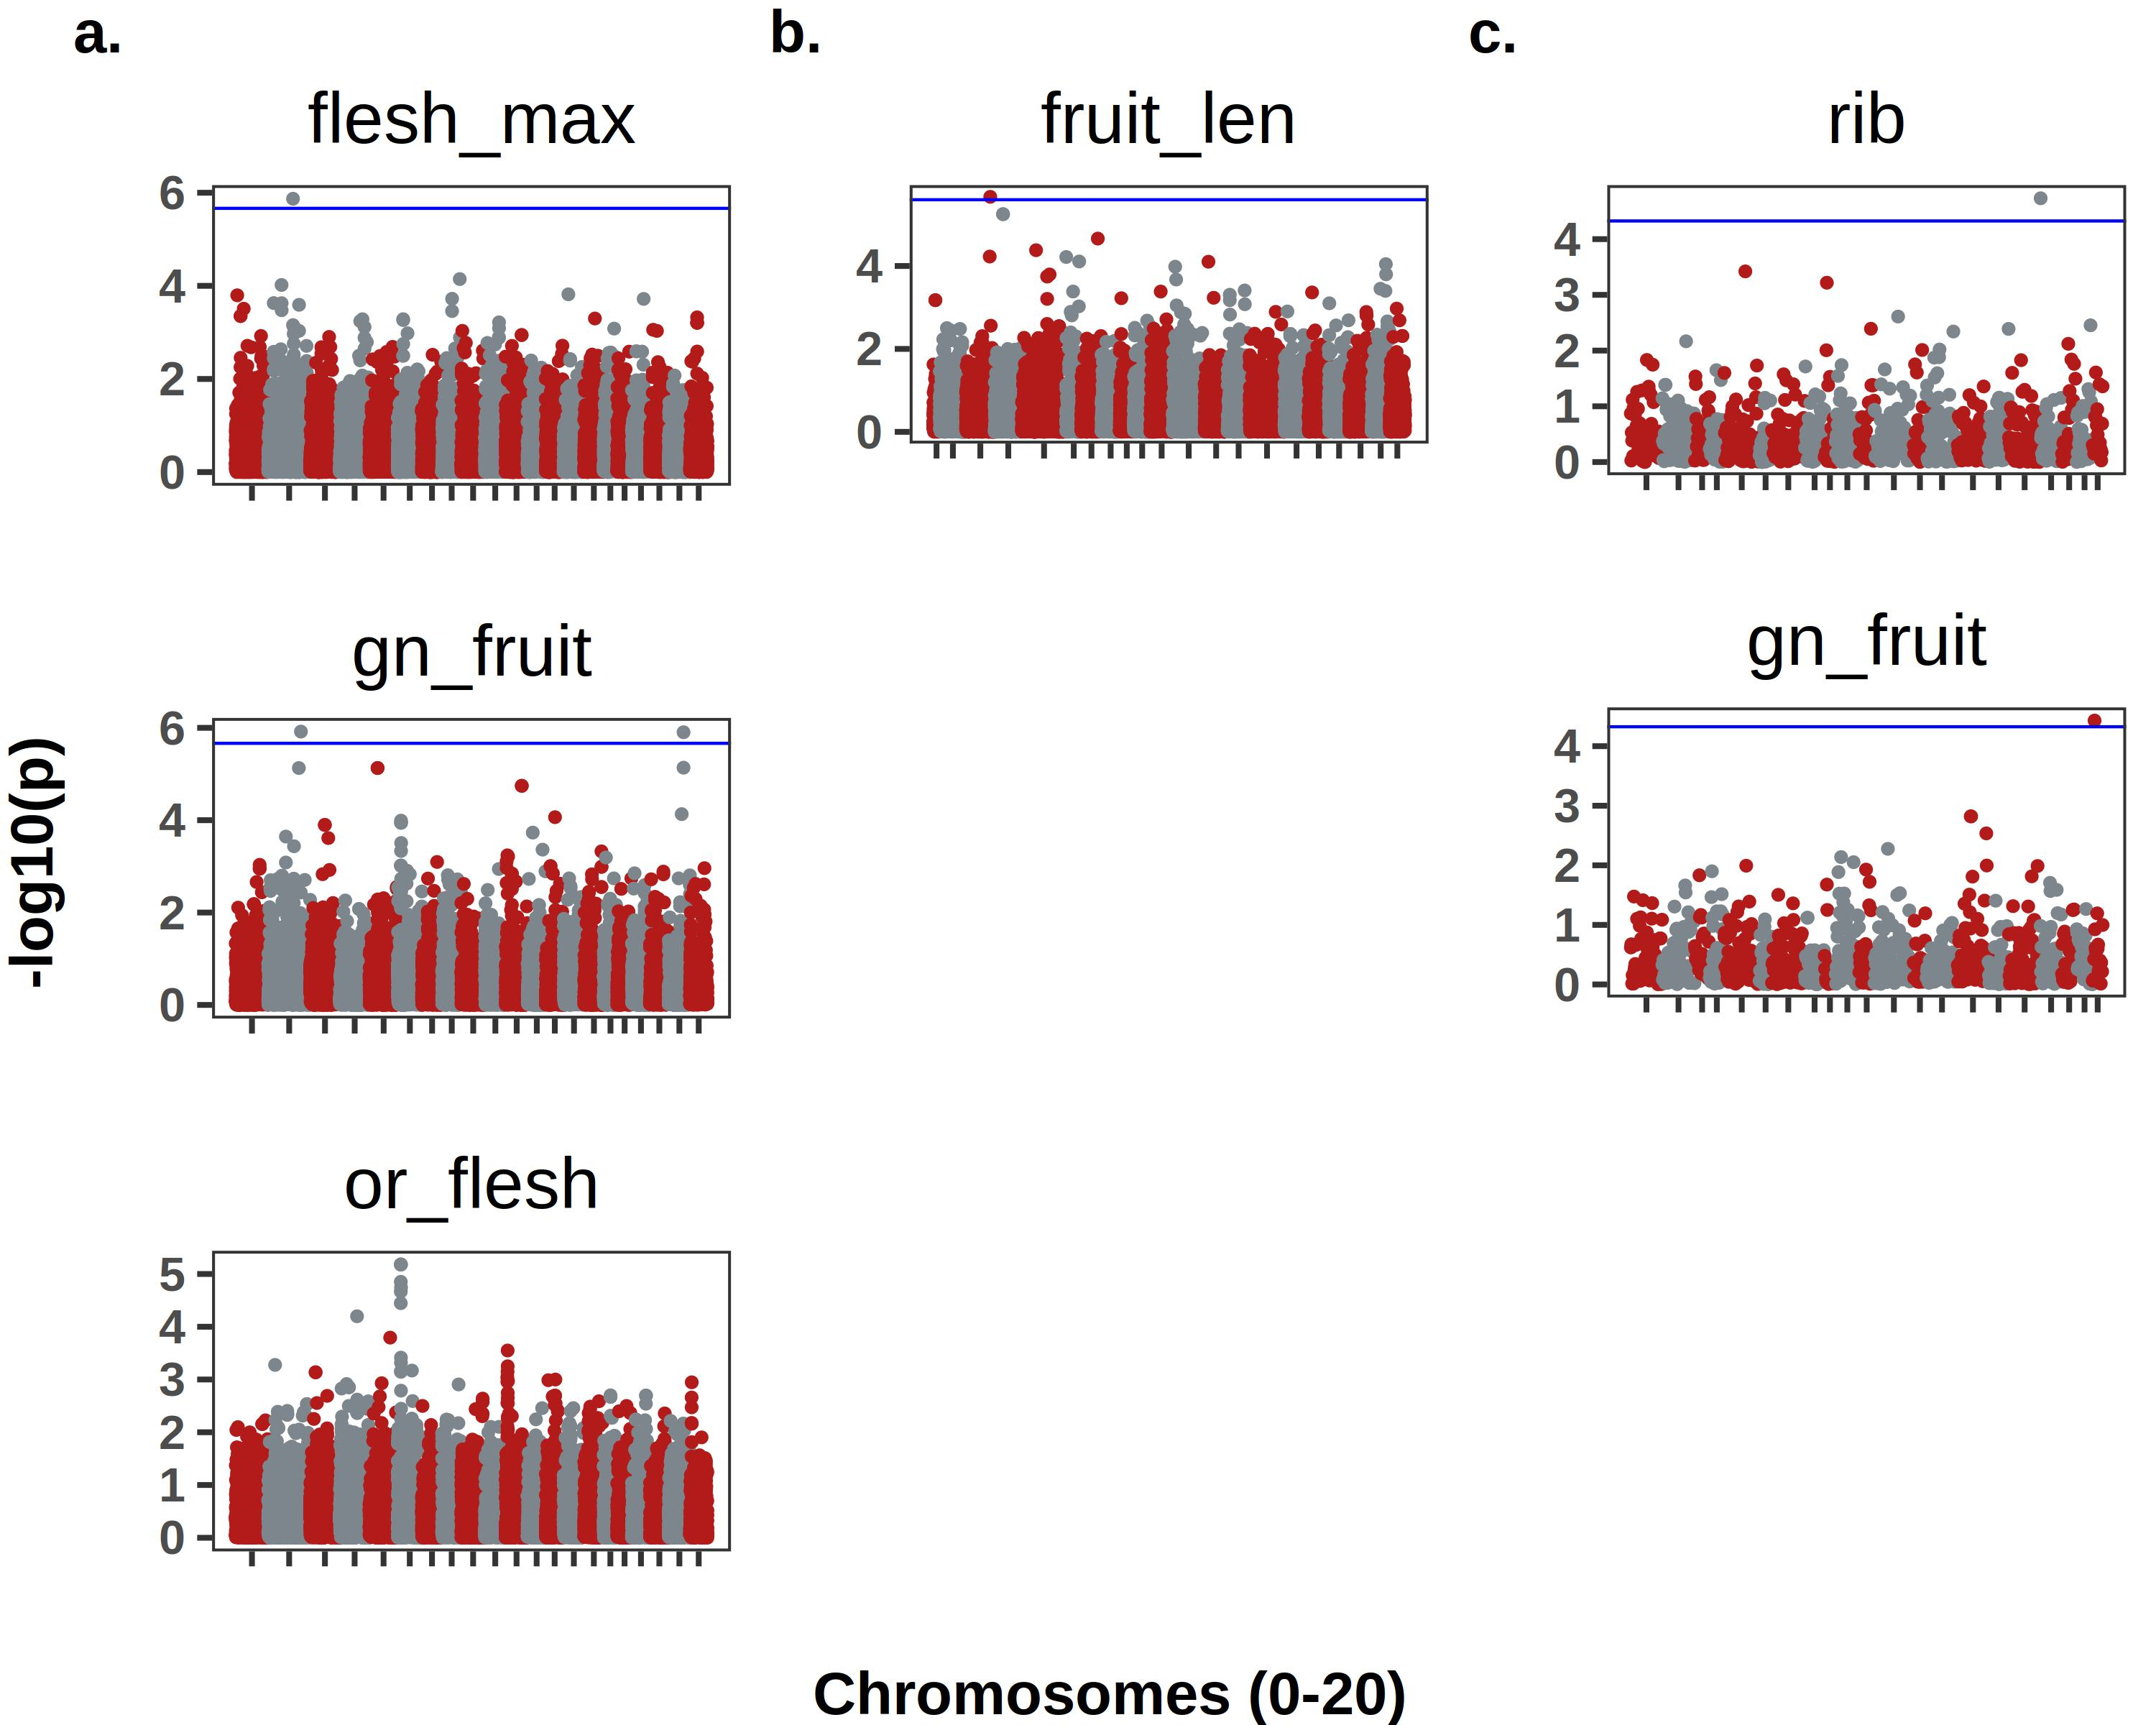
\includegraphics[width=0.8\textwidth]{../supplemental/02_supfig}% This is a *.eps file
	\end{center}
	\caption{GWAS results for \textbf{Panel a.} \textit{C. pepo}, \textbf{Panel b.} \textit{C. moschata}, and \textbf{Panel c.} \textit{C. maxima.}\label{fig:2}}
\end{figure}

\clearpage

\begin{figure}[h]
	\begin{center}
		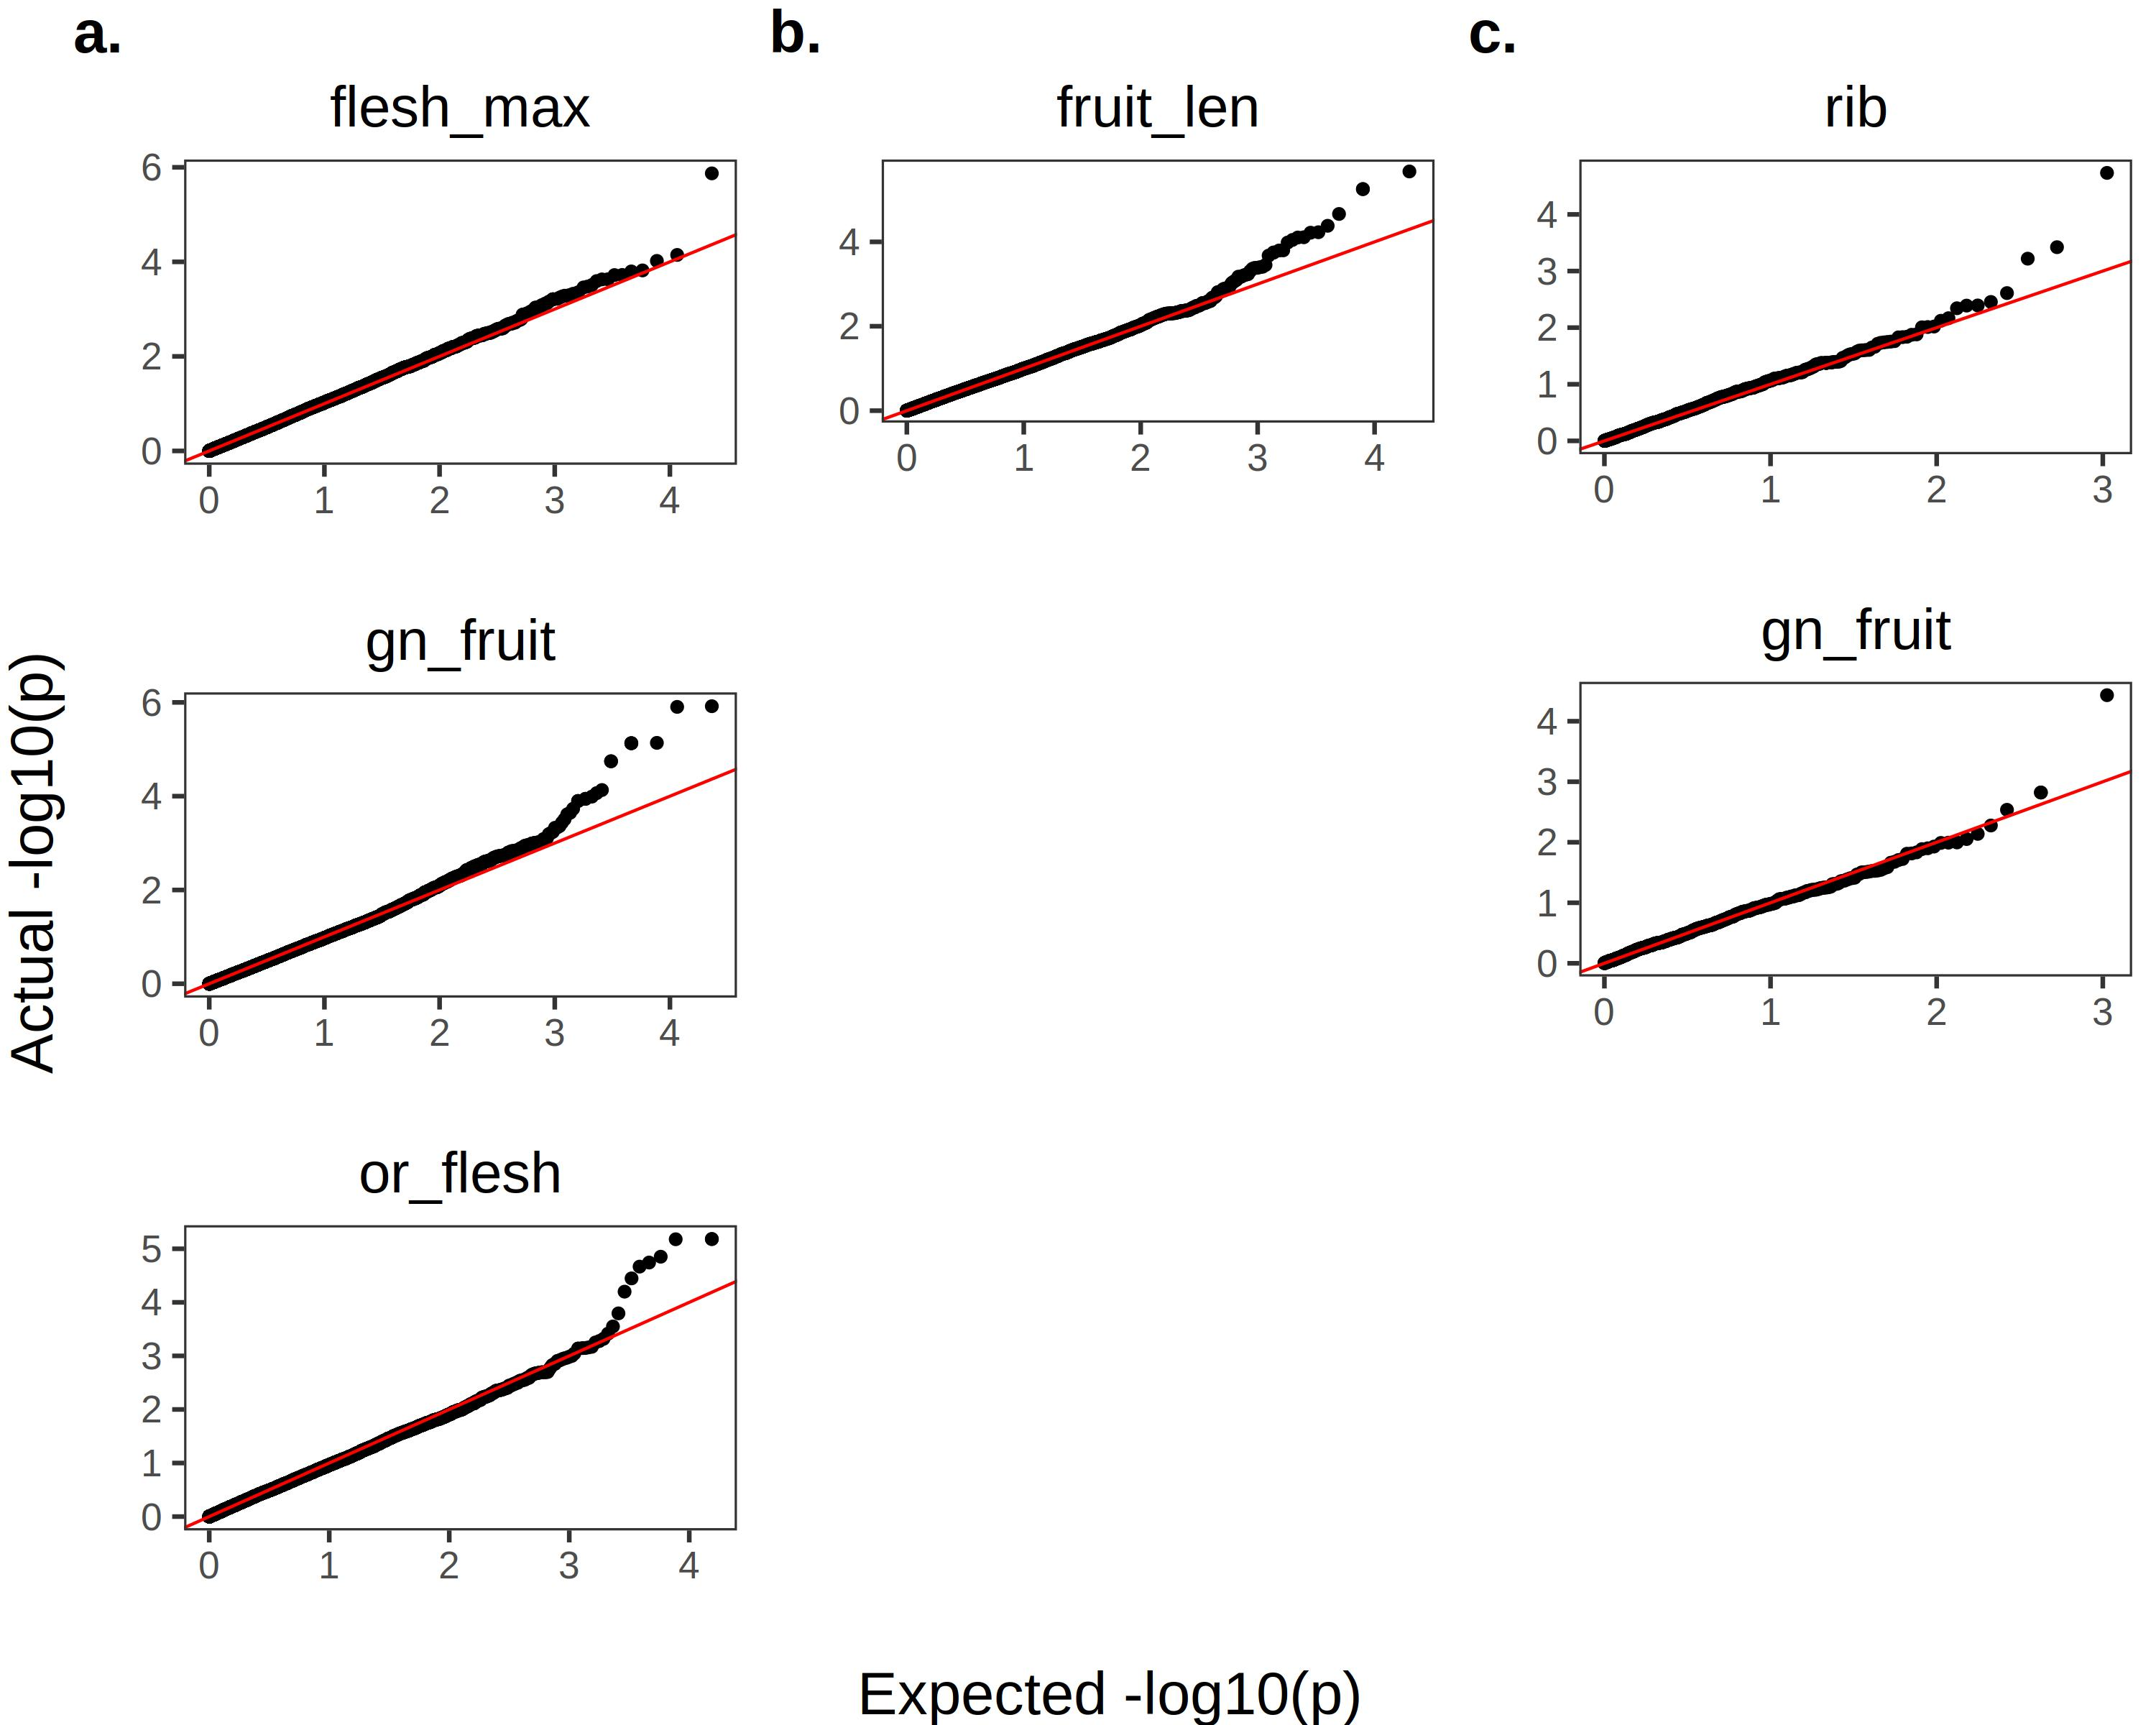
\includegraphics[width=0.8\textwidth]{../supplemental/03_subfig}% This is a *.eps file
	\end{center}
	\caption{Q-Q plots for GWAS results for \textbf{Panel a.} \textit{C. pepo}, \textbf{Panel b.} \textit{C. moschata}, and \textbf{Panel c.} \textit{C. maxima.}\label{fig:2}}
\end{figure}

\newpage

\subsection{Tables}
\begin{table}[ht]
	\centering
	\begin{tabular}{lllrl}
		\hline
		{\bfseries Trait} & {\bfseries Species} & {\bfseries Chrom} & {\bfseries Pos} & {\bfseries Alleles} \\ 
		\hline
		plant\_type & \textit{C. pepo} & 6 & 3962527 & G/C \\ 
		 &  & 10 & 3507098 & C/T \\ 
	 	&  & 10 & 3507179 & G/T \\ 
		&  & 10 & 3507087 & A/G \\ 
		 &  & 10 & 3507387 & C/T \\ 
		\hline
		plant\_type2 & \textit{C. pepo} & 10 & 679593 & A/C \\ 
		& & 10 & 753000 & T/C \\ 
		 & & 10 & 768265 & T/C \\ 
		 &  & 10 & 666810 & T/C \\ 
		 &  & 10 & 974041 & G/A \\ 
		\hline
		gn\_fruit & \textit{C. pepo} & 1 & 17395123 & C/T \\ 
		 &  & 19 & 6509248 & A/G \\ 
		 &  & 19 & 6509202 & T/C \\ 
		&  & 1 & 16658797 & G/C \\ 
		 &  & 4 & 5142030 & C/T \\ 
		\hline
		or\_flesh & \textit{C. pepo} & 5 & 1075625 & A/T \\ 
		 & & 5 & 1075652 & T/G \\ 
		 &  & 5 & 1074883 & T/C \\ 
		 &  & 5 & 1072306 & G/T \\ 
		 &  & 5 & 1115573 & C/T \\ 
		\hline
		flesh\_max & \textit{C. pepo} & 1 & 10063336 & C/T \\ 
		 &  & 7 & 9444225 & T/A \\ 
		& & 1 & 5697024 & C/T \\ 
		 & & 13 & 2248185 & G/A \\ 
		 &  & 0 & 1463850 & G/A \\ 
		\hline
		fruit\_len & \textit{C. moschata}& 2 & 9116220 & T/C \\ 
		 &  & 3 & 5539269 & T/A \\ 
		 &  & 3 & 5539270 & T/A \\ 
	 	&  & 6 & 10461612 & C/T \\ 
		&  & 4 & 6338885 & C/T \\ 
		\hline
		rib & \textit{C. maxima} & 17 & 76012 & T/C \\ 
		 & & 4 & 8332568 & C/T \\ 
		 &  & 8 & 1759117 & A/T \\ 
		 & & 11 & 6776288 & A/G \\ 
		 &  & 19 & 8123733 & A/C \\ 
		\hline
		gn\_fruit & \textit{C. maxima} & 20 & 1087480 & G/A \\ 
		 &  & 14 & 9051301 & G/T \\ 
		 &  & 14 & 9051304 & A/T \\ 
		 &  & 14 & 14410557 & C/T \\ 
		 & & 11 & 3829766 & C/T \\ 
		\hline
	\end{tabular}
	\caption{The position and allele are shown for the top five association results for each trait for which there was a GWAS signal.}
\end{table}
\end{document}
